\documentclass{beamer}
\usepackage{graphicx}
\usetheme{Madrid}

% Title page information
\title{COMP 354 Iteration 1 Eternity Project}

\author
{
Team I
}

\institute{Concordia University}
\date{Friday June 5, 2020}

\begin{document}

\frame{\titlepage}

\begin{frame}
\frametitle{Overview}
\tableofcontents
\end{frame}

\section{Team}




\begin{frame}
\frametitle{The Team}
	%\bigskip
  \hfil\hfil
\includegraphics[width=2cm]{Avnish}
  \hfil\hfil
    
\includegraphics[width=2cm]{Swati}
    \hfil\hfil
    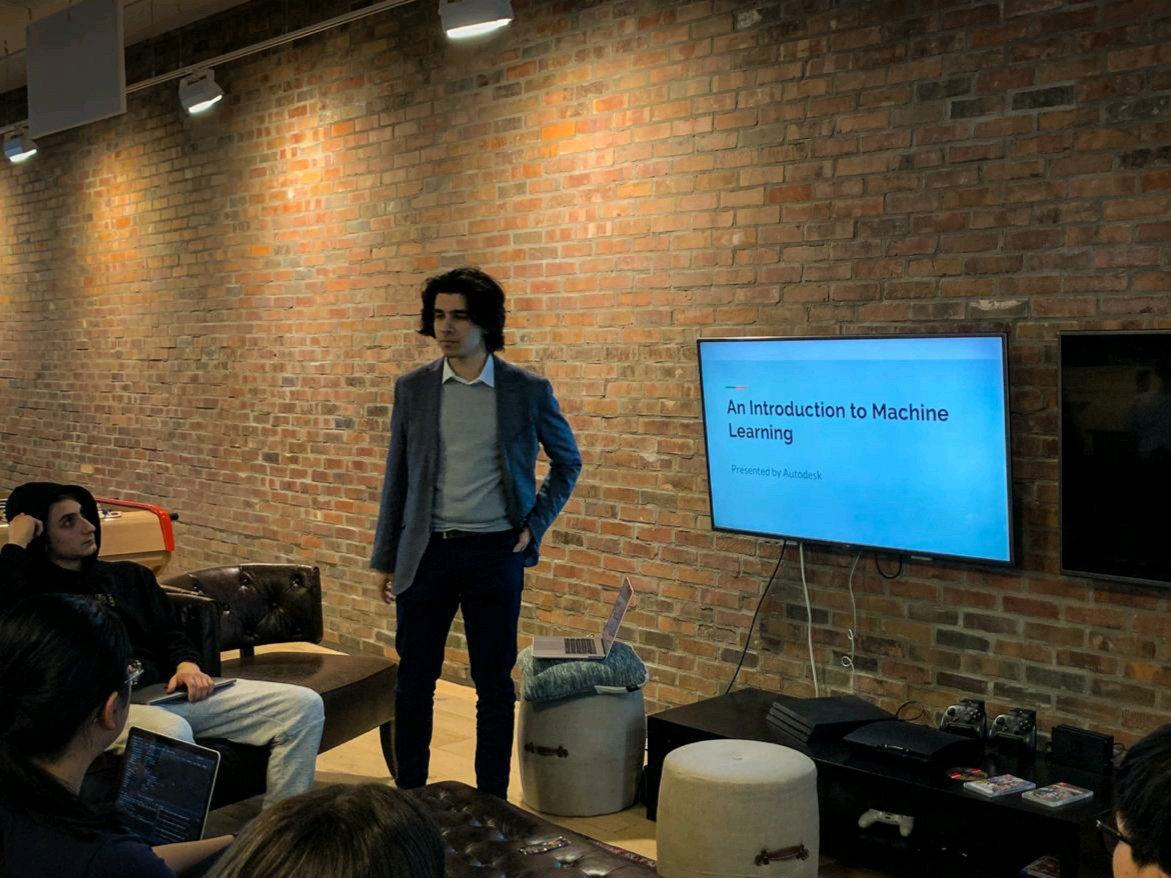
\includegraphics[width=2cm]{Emanuel}
    \newline
  \null\hfil\hfil\makebox[2cm]{Avnish: sinh(x)}
    \hfil\hfil\makebox[2cm]{Swati: $e^{x}$}  
     \hfil\hfil\makebox[2cm]{Emanuel: $log_{10}$(x)} 
    
    \bigskip
    
  \hfil\hfil
\includegraphics[width=1.5cm]{Clement}
  \hfil\hfil
    
\includegraphics[width=1.5cm]{Nguyen}
    \hfil\hfil
    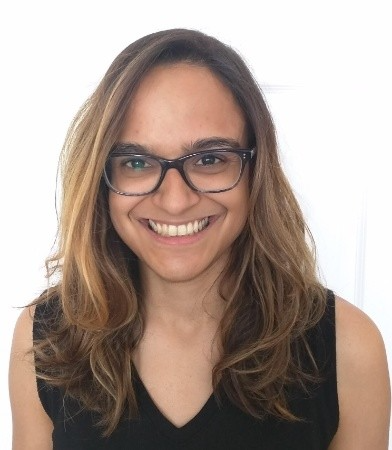
\includegraphics[width=1.5cm]{Tara}
    \newline
  \null\hfil\hfil\makebox[2cm]{Clément: $10^{x}$}
    \hfil\hfil\makebox[2cm]{Nguyen: MAD}  
     \hfil\hfil\makebox[2cm]{Tara: $x^y$} 
     \bigskip
      \bigskip
      
           \hfil\hfil
\includegraphics[width=1.5cm]{Anik}\newline
  \null\hfil\hfil\makebox[2cm]{Anik: sin(x)}\newline
\end{frame}

  \begin{frame}
\frametitle{Team Roles}
\small
\begin{table}
\begin{tabular}{l | c | c | c | c }
Name & Primary Role and Responsibility & Secondary Role \\
\hline
Hong Phuc & GUI and Web application,& Implementation of\\
& prototyping & new technologies\\
\hline
Swati & Organizing and planning agenda& High-level vision, \\
& for team meetings & scope management\\
\hline
Anik & Set up of initial repository& Questions regarding\\
& GUI for local application & the Python ecosystem\\
\hline
Avnish & Technical Writer & Latex \\
\hline
Clément & Major presenter, & Best practices, \\
& quality control  & PEP documentation\\
\hline
Tara & Minor presenter, & Ensuring requirements \\
& Team liason  & are followed\\
\hline
Emmanuel & Technical writer, &  Algorithm optimization\\
& subject matter expert  & \\
& for math algorithms  & \\
\end{tabular}
\end{table}
\end{frame}

\begin{frame}
\frametitle{Collaboration patterns:\\ Managing the project}
\begin{itemize}
 \item Regular meetings once a week
 \item Agenda
   \begin{itemize}
   \item Meeting transcriber ensures that discussions are on track
   \end{itemize}
   \item Questions are gathered by the meeting transcriber
   \item Status Update: done, doing, to-do
\end{itemize}
\end{frame}

\begin{frame}
\frametitle{Collaboration Patterns: \\ Centralizing work product management}
\begin{itemize}
 \item Focus on real-time information and feedback
 \item Discord
 \item Google Drive
 \item GitHub
  \begin{itemize}
   \item Quality Control: protected branches
     \begin{itemize}
        \item Staging branch
    \end{itemize}
   \item Required asymmetric code reviews
  \end{itemize}
\end{itemize}
\end{frame}


%Slide for future directions
\begin{frame}
\frametitle{Code Reviews}
 \begin{itemize}
  \item One individually assigned to each Pull Request
  \item Asymmetric
  \item Additional techniques used:
   \begin{itemize}
    \item Inputs and discussion from all team members encouraged
    \item Continuously enforce quality standards
   \end{itemize}
\end{itemize}
\end{frame}



\section{Requirement Gathering}

\begin{frame}
\begin{center}
\Huge Gathering Requirements
\end{center}
\end{frame}


% Slide for the interview questions
\begin{frame}
\frametitle{Interview Questions}
\begin{itemize}
 \item Demographic of people who use a calculator
  \begin{itemize}
   \item Professional/educational background
   \item Calculator Usage
  \end{itemize}
 \item User needs
  \begin{itemize}
   \item Degree of precision
   \item Input box vs. button selection
   \item Numeral system required
  \end{itemize}
 \item Separate requirements into needs and preferences
  \begin{itemize}
   \item Ease of use
   \item Aesthetics
   \item Features
   \item Platform
  \end{itemize}
   \item Frustrations with current device
\end{itemize}
\end{frame}


%Slide for the interview model
\begin{frame}
\frametitle{Interview Model}
\begin{itemize}
 \item Hourglass
   \begin{itemize}
   \item Open-ended questions
   \item Followed by specific questions
   \item Finished with open-ended questions
  \end{itemize}
 \item Findings
  \begin{itemize}
   \item Many interviewees went back to clarify a previous question answered
  \end{itemize}
\end{itemize}
\end{frame}


  %Slide for our interview findings
\begin{frame}
\frametitle{Interview: Key findings}
\begin{itemize}
 \item Precision is extremely important
 \item Existing calculators contain a lot of unnecessary buttons and features
 \item Split findings on local or web application
  \begin{itemize}
   \item Mobility when conducting experiments or for exams
   \item Preference for desktop application when working at computer
  \end{itemize}
\end{itemize}
\end{frame}




%Slide for our use case
\begin{frame}
\frametitle{Summarized Use case}
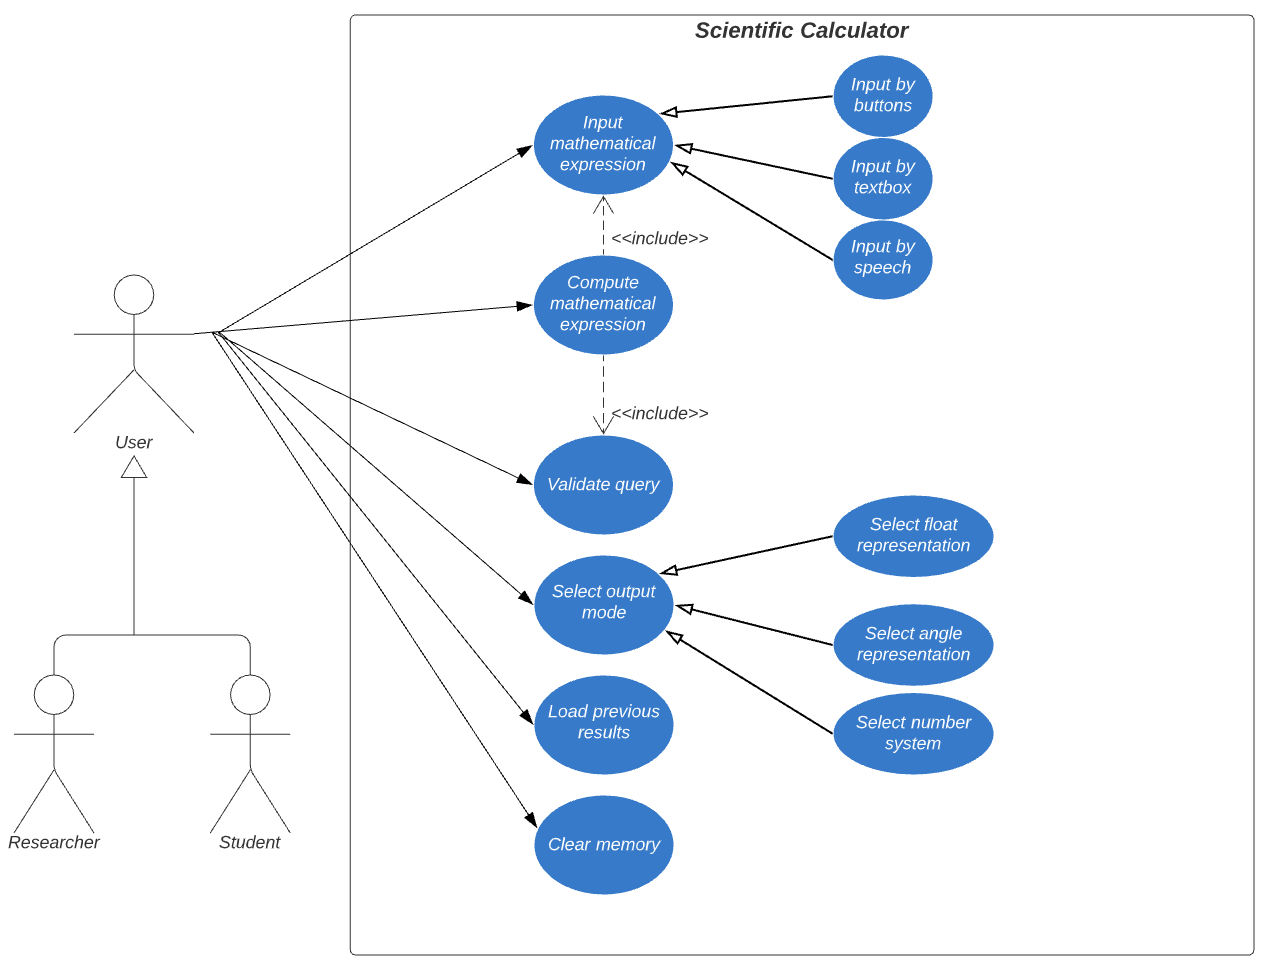
\includegraphics[scale=0.5]{Use Case}
\end{frame}


\section{Product}

\begin{frame}
\begin{center}
\Huge Product
\end{center}
\end{frame}

\begin{frame}
\frametitle{Tech Stack}
 \begin{itemize}
  \item Choice of technologies influenced by team strengths and user requirements
  \item Python: familiar \& versatile
   \begin{itemize}
    \item A language we were all comfortable with
    \item Rapid iterations
    \item Option of a GUI vs. CLI calculator
    \item Native language recognition libraries
   \end{itemize}
  \item Keeping our options open:
   \begin{itemize}
    \item Electron for a local desktop front-end
    \item Flask or nodejs for a web implementation
   \end{itemize}
  \end{itemize}
\end{frame}

\begin{frame}
\frametitle{Inclusions/Exclusions}
\begin{itemize}
 \item Information from users gave us a clear idea on what should be built
  \begin{itemize}
  \item Some ideas were not feasible in the timeframe
  \begin{itemize}
    \item Speech recognition
    \item Radian and degree conversions
  \end{itemize}
  \item Scope \& reasoning
    \begin{itemize}
    \item Essential features/functionality - for iteration 1
    \item Features/functionality to be looked at a later point
  \end{itemize}
  \end{itemize}
  \end{itemize}
\end{frame}

%Slide for future directions
\begin{frame}
\frametitle{Iteration 2: Organizational improvements}
\begin{itemize}
 \item Collaboration techniques
  \begin{itemize}
   \item Buddy system
   \item Role rotation
   \item Better project \& team wiki
  \end{itemize}
\end{itemize}
\end{frame}

%Slide for future directions
\begin{frame}
\frametitle{Our Product}
\centering
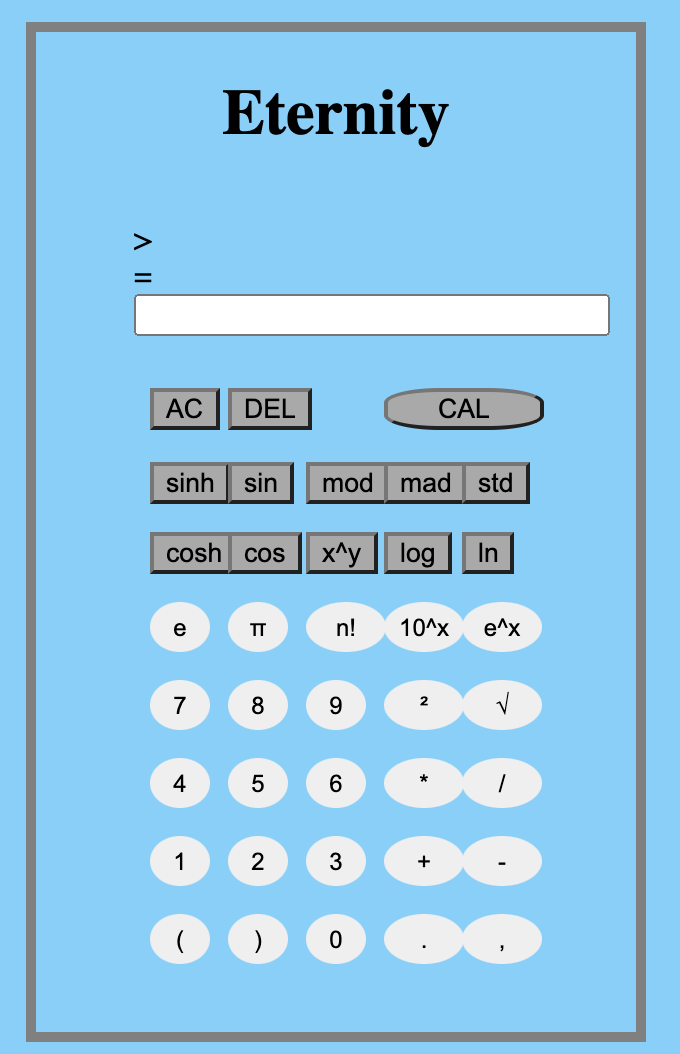
\includegraphics[scale = 0.4]{Calculator}
\end{frame}

% Slide in case we use pictures that need to be referenced
% \section{Product}
% \begin{frame}
% \frametitle{References}
% \end{frame}

\end{document}
